% !TEX root =../main.tex
\chapter{Posicionamiento mediante marcadores visuales}\label{chp:pos}


%%% Figuras %%%%
\def\figFlow{
%TODO: añadir conexión con autopiloto y pequeña descripción interna
\begin{figure}
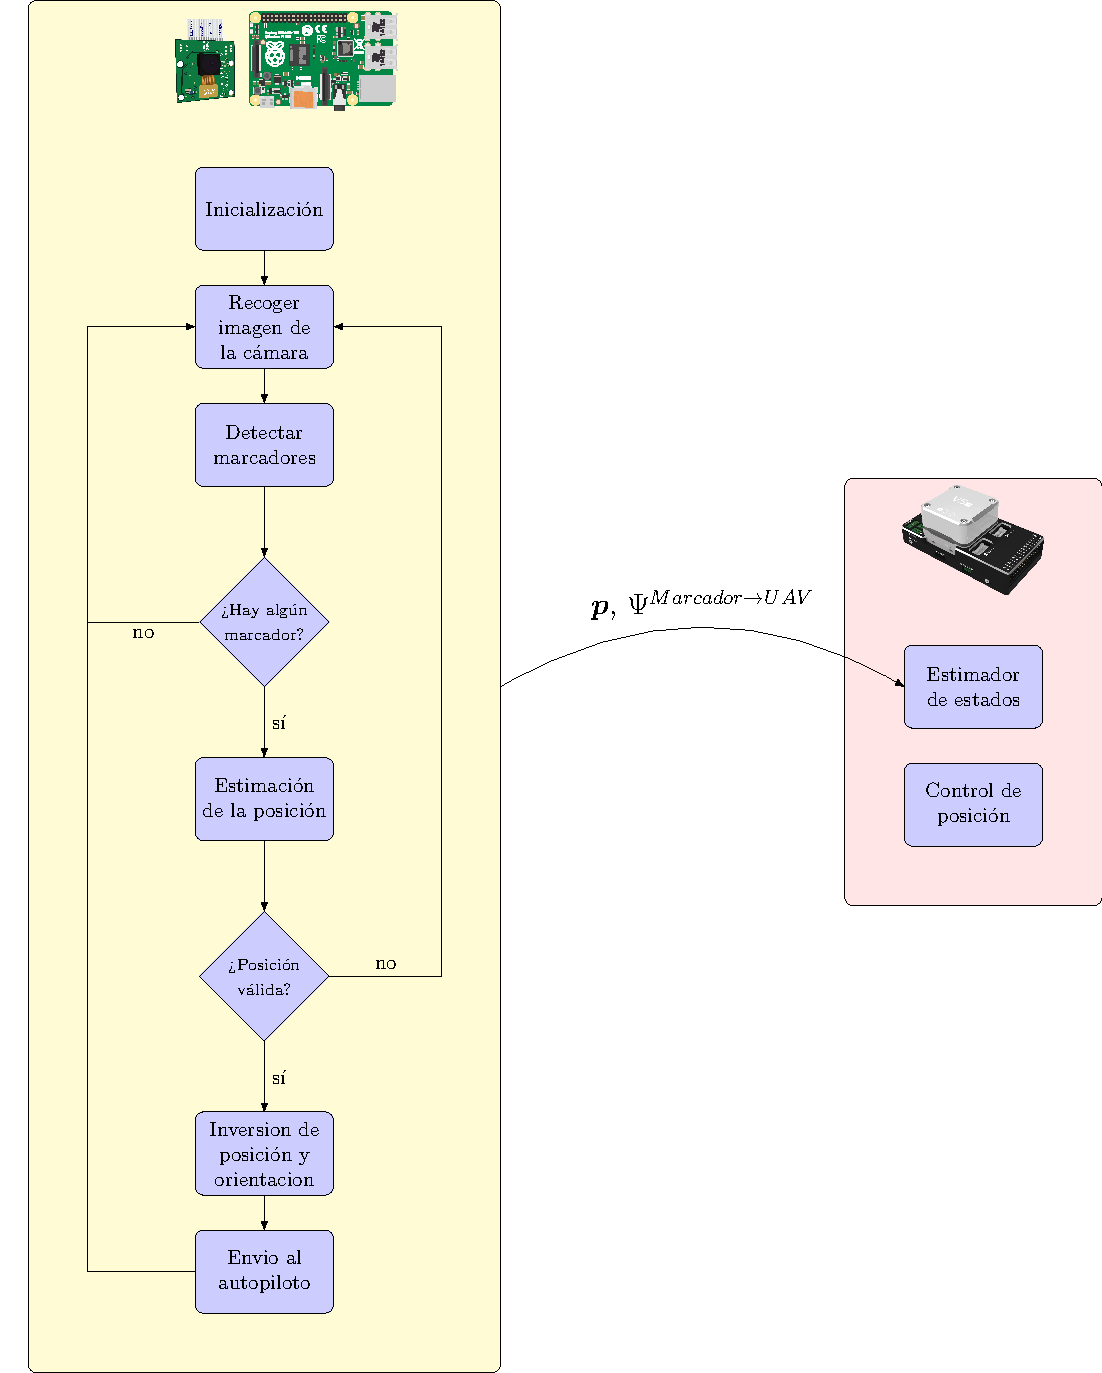
\includegraphics[width=\textwidth]{posicionamiento_marcadores/tikz/diagrama_flujo}
\caption{A la izquierda: diagrama de flujo del programa que se corre en el ordenador embebido, a la derecha: algunas de las tareas del autopiloto}
\label{fig:flow}
\end{figure}
}

\def\figEjes{
\begin{figure}
\includegraphics[width=\textwidth]{posicionamiento_marcadores/ejes}
\caption{Sistemas de referencia presentes en el problema}
\label{fig:ejes}
\end{figure}
}

\def\figComp{
\begin{figure}
	\centering
	\begin{subfigure}[t]{\textwidth}
		\centering
		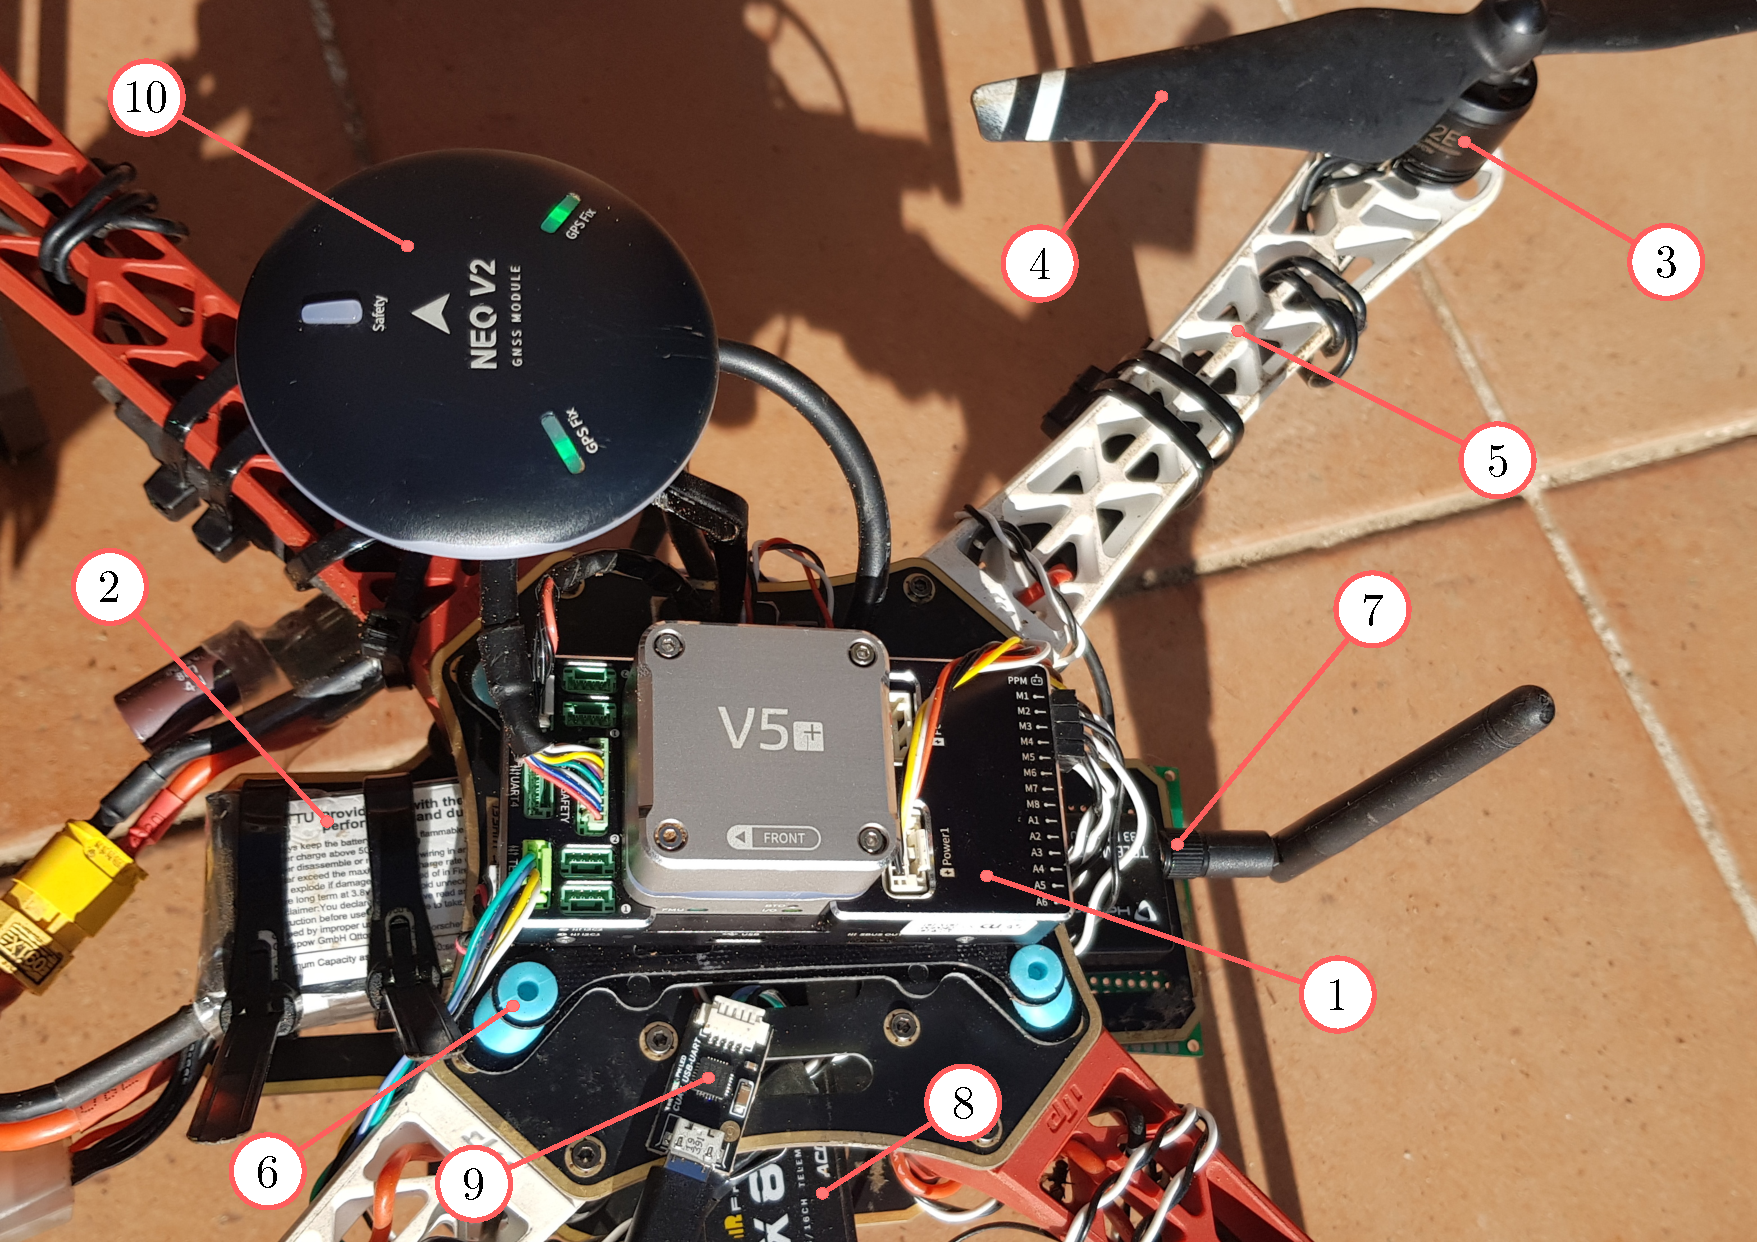
\includegraphics[width=\textwidth]{posicionamiento_marcadores/componentes.pdf}
		\caption{Vista desde arriba}\label{fig:comp1}		
	\end{subfigure}
	\quad
	\begin{subfigure}[t]{\textwidth}
		\centering
		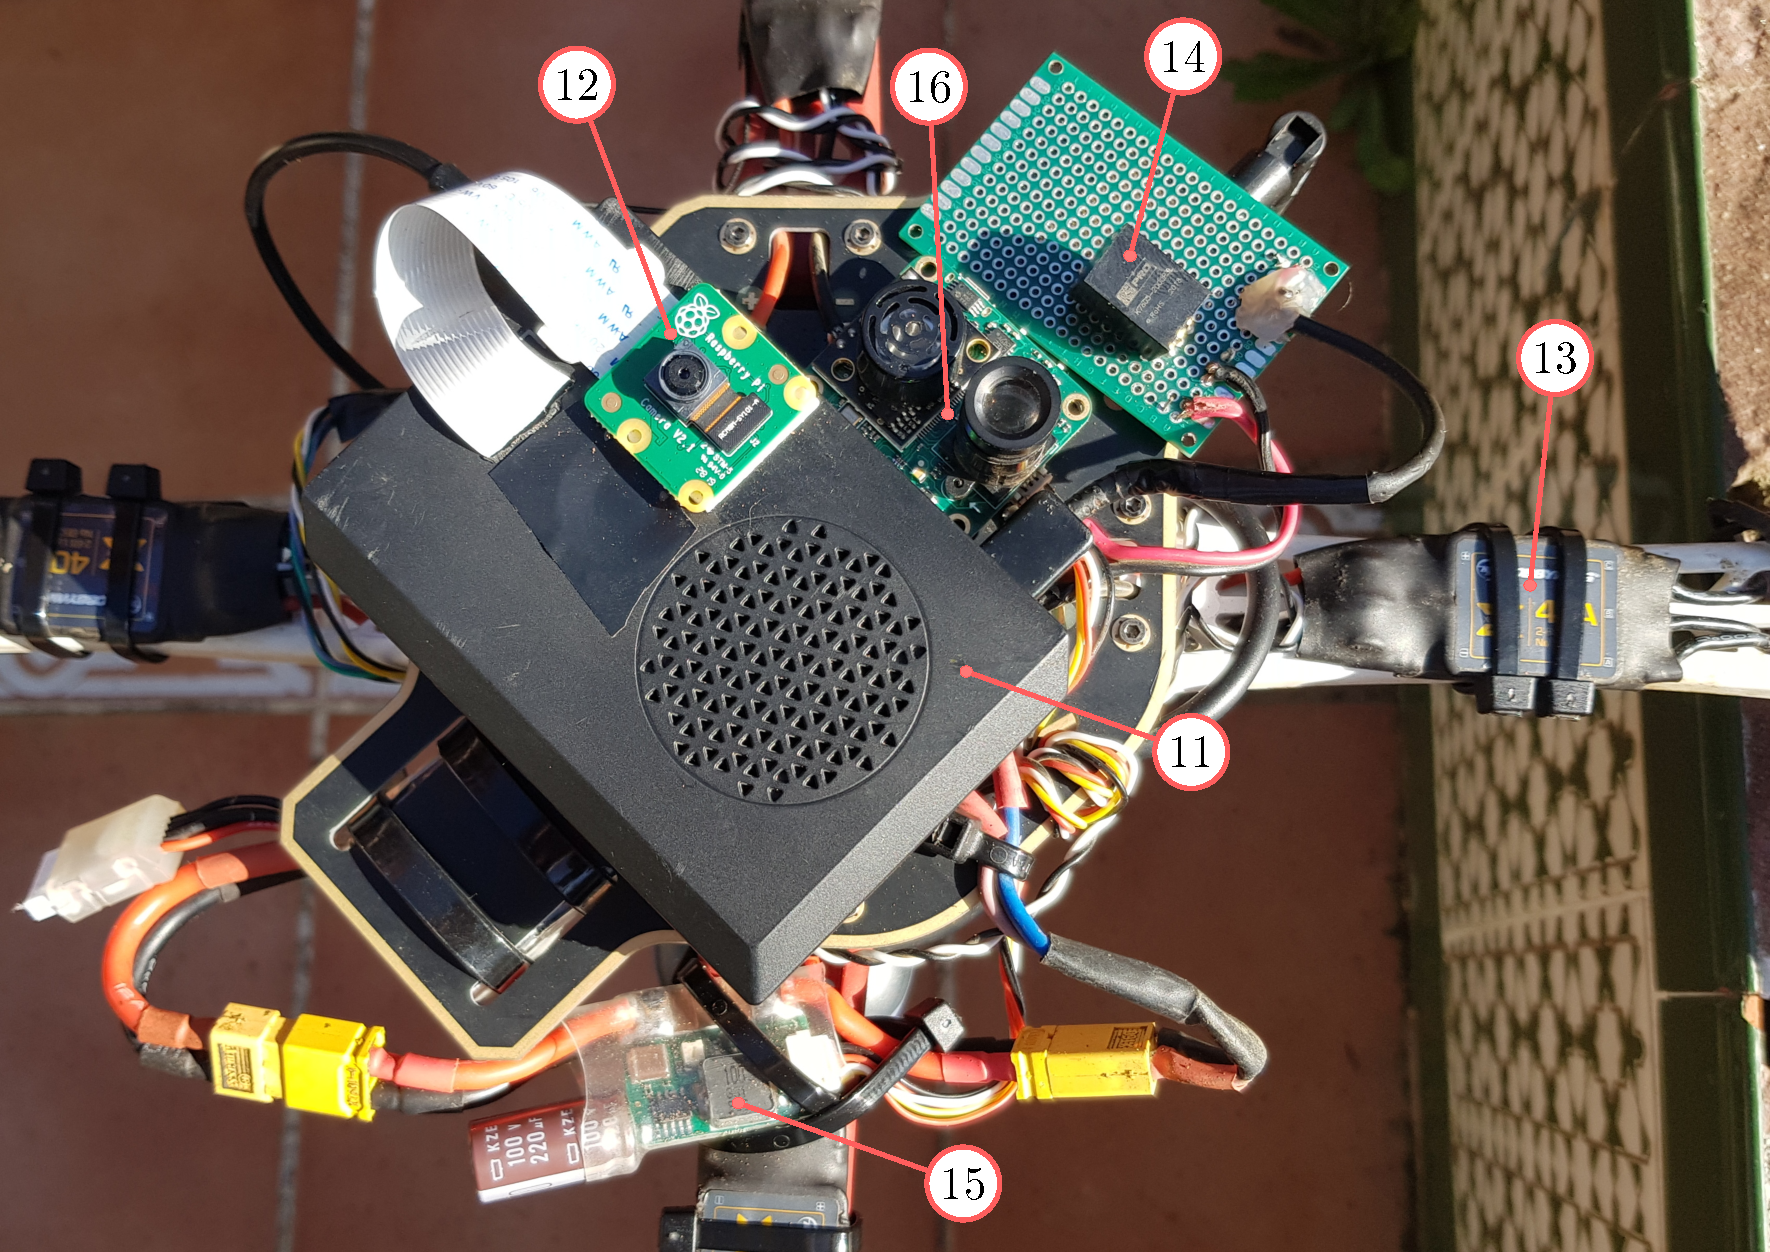
\includegraphics[width=\textwidth]{posicionamiento_marcadores/componentes_abajo.pdf}
		\caption{Vista desde abajo}\label{fig:comp2}		
	\quad
	\end{subfigure}
\caption{Componentes del quadrotor}
\label{fig:comp}
\end{figure}
}

\def\figAR{
\begin{figure}
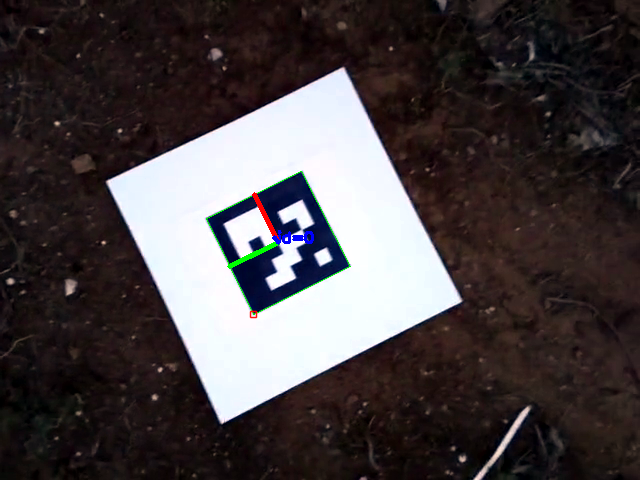
\includegraphics[width=0.5\textwidth]{posicionamiento_marcadores/image1775_white_bal.png}
\caption{Superposición de los ejes de referencia del marcador y del cuadrilátero que lo rodea (trazado en verde)}
\label{fig:AR}
\end{figure}
}

\def\figExpA{
\begin{figure}
	\centering
	\begin{subfigure}[t]{\textwidth}
		\centering
		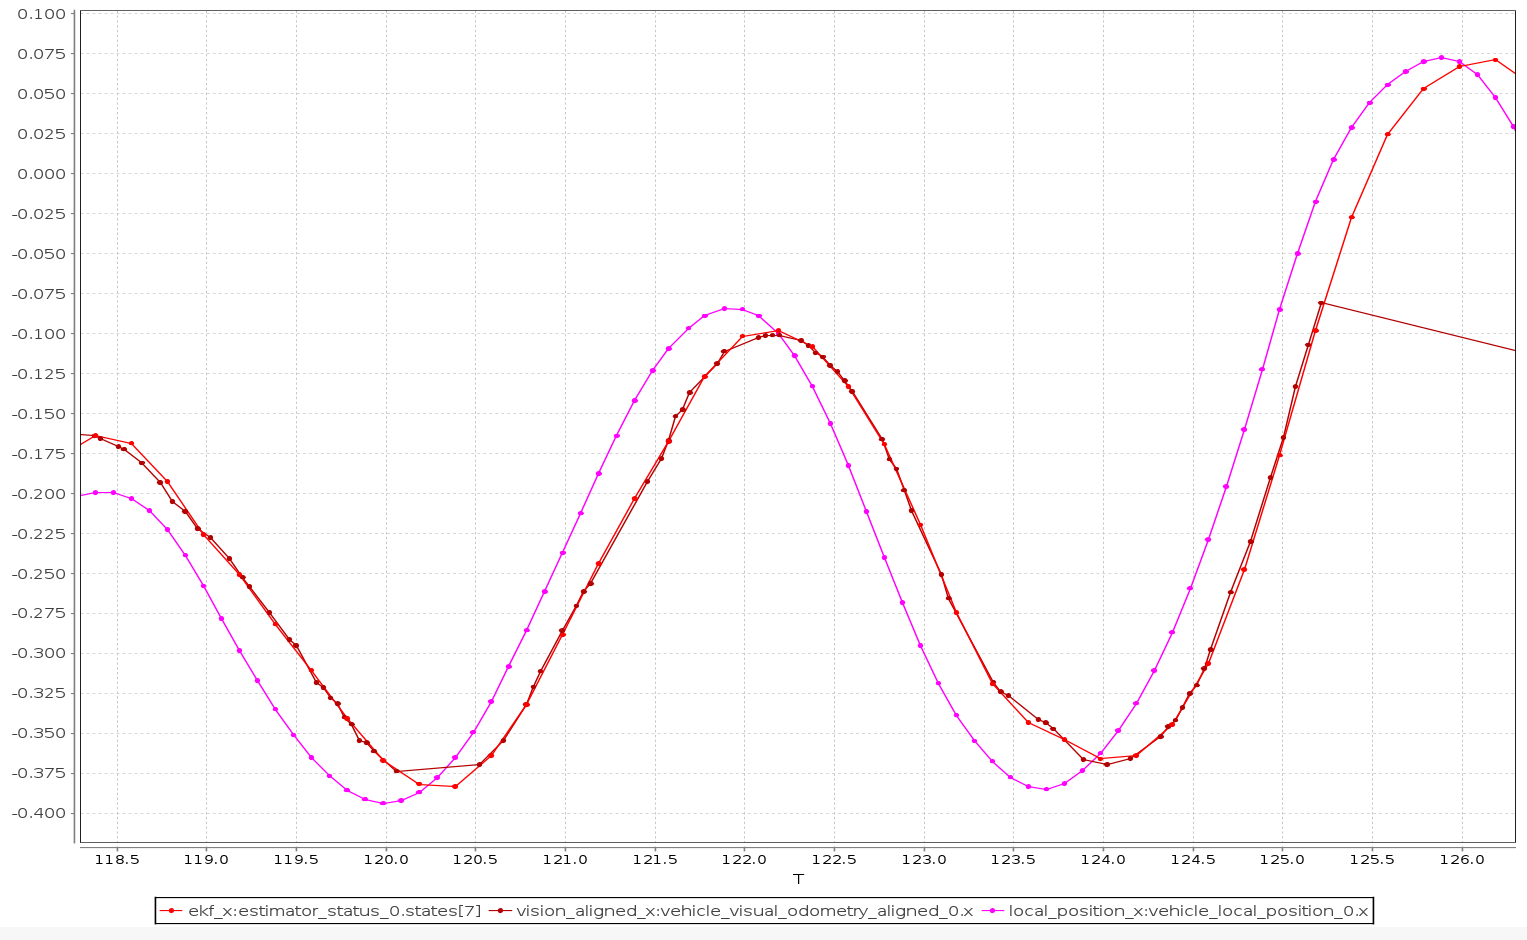
\includegraphics[width=\textwidth]{posicionamiento_marcadores/alttitude_px}
		\caption{$P_x$}		
	\end{subfigure}
	\quad
	\begin{subfigure}[t]{\textwidth}
		\centering
		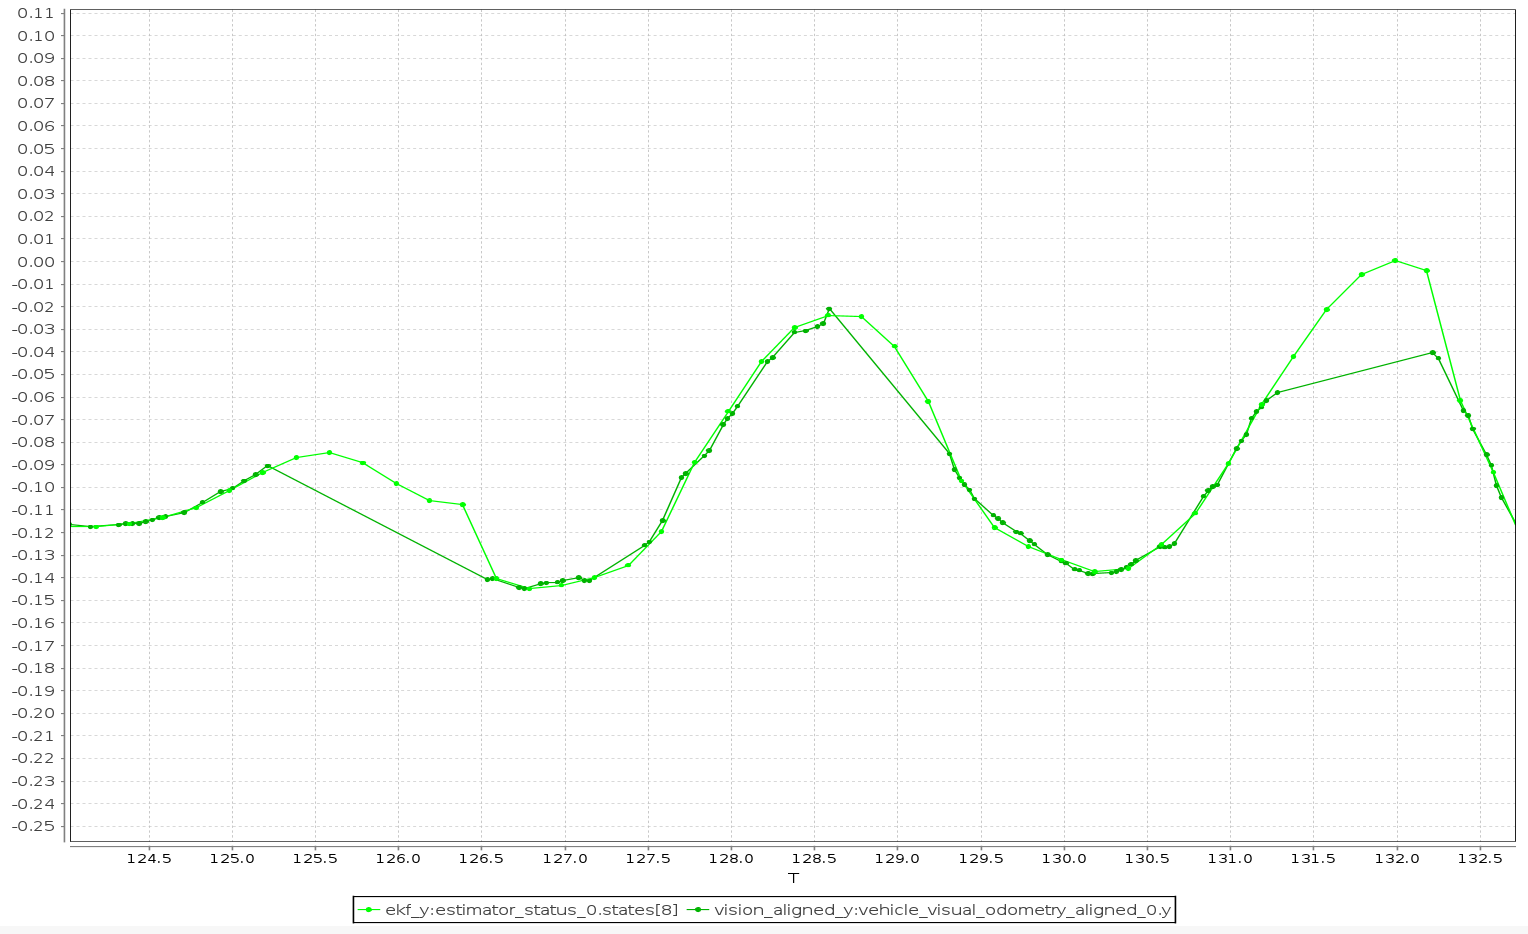
\includegraphics[width=\textwidth]{posicionamiento_marcadores/alttitude_py}
		\caption{$P_y$}		
	\quad
	\end{subfigure}
\caption{Modo altitude}
\label{fig:expA}
\end{figure}
}

\def\figExpB{
\begin{figure}
	\centering
	\begin{subfigure}[t]{\textwidth}
		\centering
		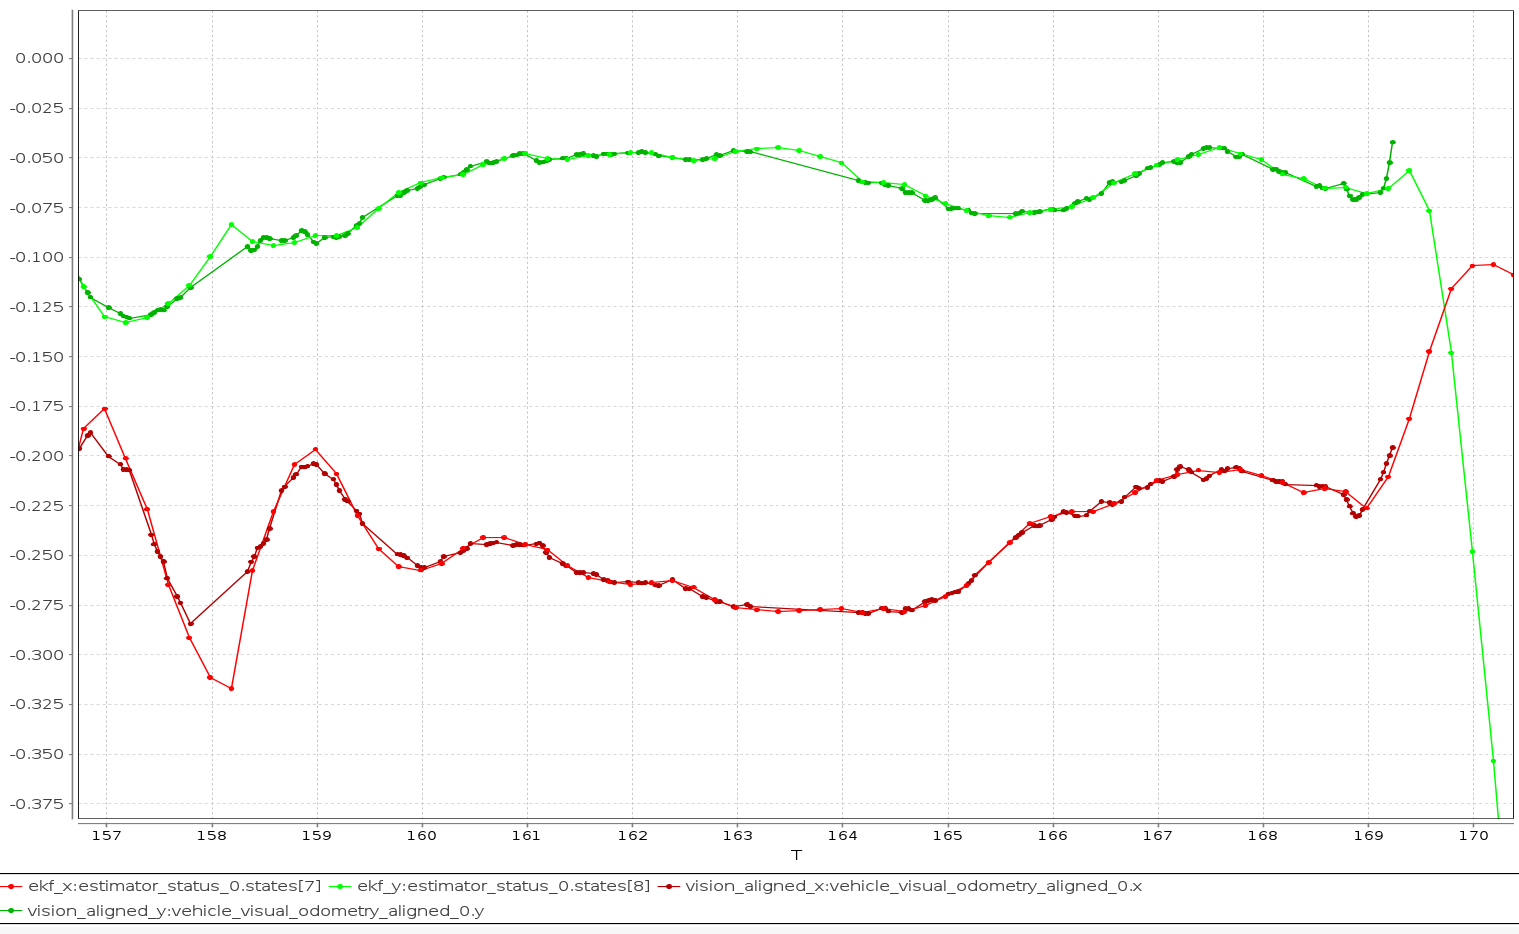
\includegraphics[width=\textwidth]{posicionamiento_marcadores/position_px_py}
		\caption{$P_x$ y $P_y$}
	\end{subfigure}
	\quad
\caption{Modo position}
\label{fig:expB}
\end{figure}
}

\def\figAruco{
\begin{figure}
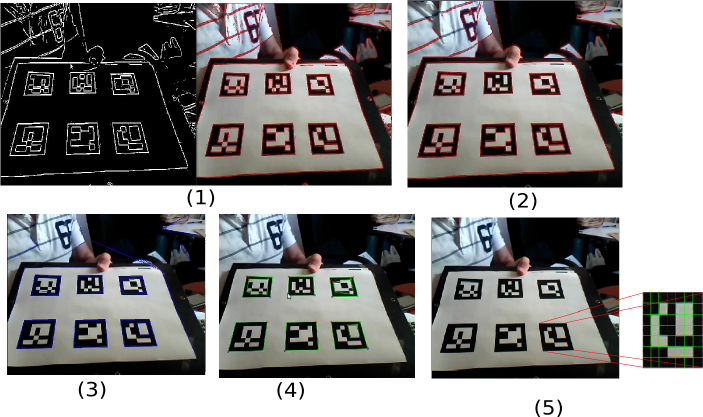
\includegraphics[width=\textwidth]{posicionamiento_marcadores/aruco_paper.png}
\caption{Pasos intermedios en el proceso de detección de marcadores Aruco. Fuente \cite{aruco2014}}
\label{fig:Aruco}
\end{figure}
}


% Más concretamente la precisión que se busca es centimétrica, pensando en coger un objeto metálico de manera autónoma con un imán colgando del UAV

%\lettrine[lraise=-0.1, lines=2, loversize=0.2]{C}{onseguir} con precisión la posición de un vehículo aéreo no tripulado es bastante deseable. En la introducción se comentó aplicaciones como la manipulación de objetos o la navegación cerca de obstáculos. En este cápitulo se explica que para conseguirlo se ha construido un quadrotor con los componentes necesarios para detectar un marcador visual y cómo se ha programado un ordenador embebido en el quadrotor para que procese dicho marcador. 
\lettrine[lraise=0.1, lines=2, loversize=0.1]{C}{onseguir} con precisión la posición de un vehículo aéreo no tripulado es bastante deseable. En la introducción se comentó aplicaciones como la manipulación de objetos o la navegación cerca de obstáculos. En este capítulo se explica que para conseguirlo, se ha construido un quadrotor con los componentes necesarios para detectar un marcador visual. Además, se comenta cómo se ha programado un ordenador embebido para que procese dicho marcador. 

\section{Componentes}
Para elegir los componentes se ha tenido en cuenta que no estén discontinuados, para comprar posibles recambios, la rapidez de llegada ya que todos llegan por paquetería, que estén ampliamente probados, y que en la medida de lo posible estuvieran liberados tanto su software como su hardware. 
\figComp

\begin{enumerate}
\item Cuav V5+. Autopiloto corriendo PX4. Esquemáticos publicados en \href{https://github.com/ArduPilot/Schematics/tree/master/CUAV/V5_Autopilot/V5\%2B}{Github}.
\item \textit{Tattu Funfly 1500mAh}. Batería LiPo de 4 celdas.
\item \textit{DJI 2312E 800KV}. Motor sin escobillas.
\item Hélices de fibra de carbono con un diámetro 9.4 pulgadas y un paso de 5 pulgadas. Según el \href{https://www.dji.com/e305/spec}{fabricante} del motor, con esta hélice se consigue un empuje de 850 gramos alimentado a 14.8 V.
\item \textit{DJI F450}. Chasis de quadrotor de 45 cm de diagonal. 
\item Cama amortiguadora para el autopiloto\footnote{Este componente, al igual que muchos otros, fue comprado en la tienda online \textit{rc-innovations.es}}.
\item Módulo de telemetría \textit{Holybro V3}. Permite una comunicación con la estación de control terrestre.
\item Receptor \textit{X8R}. Recibe hasta 16 canales de la emisora, que este caso es una \textit{Taranis Q X7}. 
\item \textit{SILABS CP2102}. Puente USB-UART. Se conecta entre el puerto USB del ordenador embebido y el puerto UART del autopiloto.
\item CUAV NEO V2. Este incluye GNSS, magnetómetro, botón de armado, luces indicadoras y alarma sonora.

\item Raspberry Pi 4 Model B. 4 GB de RAM. Se encuentra protegida por una carcasa que incorpora un ventilador. 
\item Raspberry Pi Camera Module v2. Campo de visión horizontal de 62 grados, capaz de grabar vídeo con resolución de 1640x1232 a 40fps.
\item \textit{CUAV HV PM (High-Voltage Power Module)}. Regulador de voltaje para alimentar el autopiloto. Además, lee el voltaje y la corriente que suministra la batería. 
\item \textit{Hobbywing XRotor 40A}. Variador de velocidad o ESC. Estos están sobredimensionados ya que fabricante recomienda unos que soporten cómo mínimo una corriente de 20A.
\item \textit{RS PRO K7805-2000R3L}. Reductor de voltaje de 5V y 2A. Este se utilizará para alimentar al ordenador embebido a partir de la batería. Su voltaje permitido de entrada está entre los 8V y los 32V, lo cual es adecuado para una batería LiPo de 4 celdas. 
\item \textit{CUAV PX4FLOW 2.1}. Sensor de flujo óptico. También tiene su \href{https://github.com/PX4/PX4-Flow}{sofware} liberado y el \href{https://github.com/pixhawk/Hardware/tree/master/FLOWv1}{esquemático} de una versión anterior.
\item Extensor de piernas. Estás fueron impresas mediante la empresa \href{https://impresion3dlowcost.es/}{Impresion 3D LowCost} con un modelo tomado de la página \href{https://www.thingiverse.com/thing:915639}{Thingiverse}. Son necesarias ya que el chasis tiene unas patas demasiado cortas y no dejaban espacio para la Raspberry Pi y su cámara. 
\end{enumerate}

%TODO: Tomar foto y enumerar componentes


\section{Programa ejecutado en el ordenador embebido}
De forma resumida, la cámara, que se ha colocado en la parte inferior del quadrotor y conectada al ordenador embebido, captura imágenes de un marcador que se ha impreso y se ha colocado en el suelo. Este ordenador las procesa y genera una posición estimada del UAV con respecto al marcador, que es enviada al autopiloto a través del puerto serie. El autopiloto la fusiona en su estimador de estados y genera una posición estimada que alimenta al controlador de posición.  El controlador de posición toma esta medida y sigue la referencia. Esta última puede venir o bien del mando o del ordenador embebido el cual le indique una trayectoria.

% generando consignas de aceleración en ejes cuerpo en función de los errores de posición en ejes cuerpo
Nótese que el controlador de posición también se podría haber ubicado en el ordenador embebido, generando consignas de inclinación al autopiloto. 
La desventaja de esto es que se no se utilizan los demás sensores para el posicionamiento.
De la manera que aquí se ha implementado, si en un instante falta la medida de la visión, el autopiloto podría tomar otras como la del acelerómetro, el GPS o el flujo óptico, para fusionarlas en su estimador de estados mientras se espera a que se recupere la medida de la visión.

En la figura \ref{fig:flow} se puede ver el diagrama de flujo del programa que se corre en la Raspberry Pi, cuyos pasos se detallarán a continuación.

% TODO: Poner un trocito de código de cada programa

\figFlow

\begin{enumerate}
\item Inicialización:

	En este paso se espera a detectar el autopiloto y se leen los parámetros de un archivo dedicado a ello.

\item Recoger imagen de la cámara: 

	Este paso podría llegar a ser muy lento si no se escoge una interfaz con la cámara adecuada, por ejemplo USB. En este caso se ha escogido CSI, que lleva la imagen directamente a la GPU y esta la transfiere a la RAM mediante DMA \footnote{Para más información del proceso de captura visitar la excelente documentación de la interfaz Python de la cámara: \url{https://picamera.readthedocs.io/en/release-1.13/fov.html\#division-of-labor}}. Esta tiene la desventaja que el cable es plano y más difícil de torsionar. La ventaja es que la imagen llega a la RAM sin sin consumir tiempo de CPU permitiendo que esta haga en paralelo otras operaciones como el procesamiento de imagen.

\item Detectar marcadores: 

	El objetivo es ubicar los marcadores en la imagen (en concreto sus 4 esquinas) y extraer su identificador.  Este proceso está explicado en la sección \ref{sec:detectAruco}. 

\item Estimación de la posición:

	La estimación de la posición y la orientación se realiza tomando las esquinas de un marcador obtenido en el paso anterior. Este problema se denomina PnP (Perspectiva desde n puntos) y su solución es iterativa. Parte de que, dados unos puntos 3D en el espacio, expresados en un sistema de referencia exterior a la cámara y dada la posición de la cámara con respecto a dicho sistema de referencia, se puede predecir que posición en el plano de la imagen tendrían esos puntos al ser proyectados. Lo que se busca es exactamente lo contrario: la posición de la cámara con respecto a dicho sistema de referencia a partir de la proyección de unos puntos tridimensionales en la imagen. Lamentablemente no se puede invertir las ecuaciones y por tanto no se puede obtener una solución analítica. Para hallar la solución se recurren a algoritmos de optimización que van probando posiciones de la cámara, hacen proyecciones suponiendo esa posición y se compara con las proyecciones reales. A la diferencia de estas dos proyecciones se le denomina \textit{error de reproyección} y es el valor que se trata de minimizar. Para este proyecto este problema no se ha tenido que implementar, solo se ha tenido que llamar a la función \textit{estimatePoseSingleMarkers} de la librería Aruco, que a su vez llama a la función \href{https://docs.opencv.org/4.5.0/d9/d0c/group\_\_calib3d.html\#ga549c2075fac14829ff4a58bc931c033d}{\textit{solvePnP}} de OpenCV.

% No se han utilizado matrices de transformación homogénes porque su inversión no es igual a su traspuesta. Existe un método computacionalmente eficiente pero no es tan intuitivo https://mathematica.stackexchange.com/a/106260

\item Inversión de posición y orientación:
	\figEjes

	Como se ve en la figura \ref{fig:ejes} hay varios sistemas de referencia que entran en juego y hay que tenerlos presentes para transformar desde lo que aporta la estimación de la posición hasta lo que necesita el autopiloto. En el paso anterior, la orientación y posición que se obtiene es la del \textbf{marcador con respecto a la cámara}, es decir se obtiene $R^{C\acute{a}mara \rightarrow Marcador}$ y $p^{C\acute{a}mara \rightarrow Marcador}$. Lo primero que se realiza es buscar la orientación de la cámara con respecto al marcador. Para ello tenemos que invertir la orientación dada, la cual al ser una matriz de rotación, se puede obtener mediante su traspuesta:

	\begin{equation}
	R^{Marcador \rightarrow C\acute{a}mara } = \left(R^{C\acute{a}mara \rightarrow Marcador}\right)^T
	\end{equation}


Dicha matriz se utiliza para expresar la posición del marcador en unos ejes paralelos a los ejes del marcador. 
	\begin{equation}
	p^{C\acute{a}mara' \rightarrow Marcador} = R^{Marcador \rightarrow C\acute{a}mara} \cdot p^{C\acute{a}mara \rightarrow Marcador}
	\end{equation}
Nótese que esta posición sigue teniendo origen en la cámara, solo que ahora está rotado el sistema de referencia en el que se expresa. Lo que se quiere obtener es la posición con respecto al sistema de referencia del marcador, el cual es paralelo al que se está expresando ahora. Siempre que existen dos sistemas de referencia A y B, con la misma orientación pero ubicados en distintos puntos, se debe de negar la posición de A con respecto a B para conseguir la posición de B con respecto a A. Por esta razón la posición que finalmente se le manda al autopiloto es la negada de la obtenida en la última ecuación.   
	\begin{equation}
	p^{Marcador \rightarrow C\acute{a}mara' } = - p^{C\acute{a}mara' \rightarrow Marcador}
	\end{equation}

 En cuanto a la orientación, como se ve en la figura \ref{fig:ejes}, los ejes de la cámara y los del UAV están rotados 180\textdegree con respecto al eje z. Conociendo esto se obtiene la orientación del marcador visto desde el sistema de referencia del UAV:

	\begin{align}
	R^{UAV\rightarrow C\acute{a}mara}& = \begin{bmatrix} -1 & 0 & 0\\ 0 & -1 & 0 \\ 0 & 0 & 1 \end{bmatrix}\\
	R^{UAV \rightarrow Marcador}& = R^{UAV\rightarrow C\acute{a}mara}\cdot R^{C\acute{a}mara\rightarrow Marcador}
	\end{align}
Es muy importante que la multiplicación se realice en ese orden, ya que la multiplicación de matrices no es conmutativa. De esta manera, la rotación se realiza con respecto al eje z de la cámara, mientras que si se hubiese invertido el orden, es decir se postmultiplica a $R^{C\acute{a}mara\rightarrow Marcador}$, la rotación se hubiese hecho alrededor del eje z del marcador.
	Finalmente, esta última matriz se transpone para tener la orientación del UAV con respecto al marcador.
	\begin{align}
	R^{Marcador \rightarrow UAV}& = \left(R^{UAV \rightarrow Marcador}\right)^T
	\end{align}
	Tras expresar esta rotación en ángulos de euler, ya se podría enviar al autopiloto.
	Estos cálculos están implementados en a partir de la línea \ref{line:invertPose} del archivo \textit{marker\_vision.h} que se ha incluido en el anexo.


	
\item Envio al autopiloto: 

	La orientación y la posición son enviadas al autopiloto a través del protocolo \textit{Mavlink} utilizando la librería \textit{MAVSDK}

\end{enumerate}

Mientras tanto, en el autopiloto, una vez que las recibe, este calcula la rotación entre su orientación expresada en ejes NED y su orientación expresada en el sistema de referencia de la visión, que en este caso es el del marcador. 
\begin{align}
R^{NED \rightarrow Marcador}& =  R^{NED \rightarrow UAV} \cdot  \left(R^{Marcador \rightarrow UAV}\right)^T
\end{align}
Esta matriz se utiliza para transformar la posición que le llega de la visión, expresándola en ejes NED (norte, este y abajo).
\begin{align}
p^{NED' \rightarrow UAV}& = R^{NED \rightarrow Marcador} \cdot p^{Marcador \rightarrow UAV}
\end{align}
Siendo $NED$ el sistema de referencia centrado en la posición que partió el UAV y $NED'$ uno que es paralelo a este último pero centrado en el marcador.
Que tengan esta orientación es importante, ya que el EKF en su fase de predicción, utilizando el acelerómetro y la orientación estimada, expresa su posición en ejes NED.
Estos cálculos se pueden ver el código \ref{cod:invPX4} donde se han extraído algunos fragmentos de PX4. 

\begin{codigo}[label=cod:invPX4]{Rotación en PX4 de la posición suministrada por la visión}
En el archivo \href{https://github.com/PX4/PX4-ECL/blob/ec934908900b23ee273d1a9f82364b7b38423200/EKF/ekf\_helper.cpp\#L1460}{\textit{ekf\_helper.cpp}} se calcula la rotación que hay que aplicarle a la posición:
\begin{minted}[firstnumber=1460]{c++}
    const Quatf q_error((_state.quat_nominal * _ev_sample_delayed.quat.inversed()).normalized());
    _R_ev_to_ekf = Dcmf(q_error);
\end{minted}
En el archivo \href{https://github.com/PX4/PX4-ECL/blob/ec934908900b23ee273d1a9f82364b7b38423200/EKF/control.cpp\#L273}{\textit{control.cpp}} se aplica dicha rotación:
\begin{minted}[firstnumber=273]{c++}
    ev_pos_meas = _R_ev_to_ekf * ev_pos_meas;
    ev_pos_var = _R_ev_to_ekf * ev_pos_var * _R_ev_to_ekf.transpose();
\end{minted}
\end{codigo} 

Con estas transformaciones ya se podría fusionar la medida de la visión. Así, se generarán unos estados estimados que serán tomados por los controladores de PX4. Como se explicó en \cite{arias2019control} estos forman una estructura en cascada cuyo controlador de mayor nivel es el de posición. 


\section{Detección de marcadores Aruco} \label{sec:detectAruco}
	Los marcadores Aruco fueron creados por el departamento Aplicaciones de la Visión Artificial de la universidad de Córdoba. Estos pertenecen a la categoria de marcadores visuales planos y cuadrados y su misión es ofrecer su posición relativa a la cámara además de identificarlo. 
	Como se aprecia en la figura \ref{fig:Aruco}, estós son cuadrados que tienen en su interior unas figuras que codifican un número en binario. Estas últimas solo se utilizan en la identificación, mientras que le borde exterior es el que se usa para la estimación de la posición. Este proceso está explicado en \cite{aruco2014} pero aquí se hará un resumen del mismo. Los pasos principales son los siguientes:
\figAruco
\begin{itemize}
\item Detección de bordes. 

	Se denomina borde a la línea que separa 2 regiones, en el caso de los marcadores estas regiones son las zonas blancas y las negras. Aunque no es usado  en este caso por su coste computacional, el algoritmo de Canny puede servir para explicar un método de detección de bordes. 
	Quienes no estén familiarizados con el campo de la visión artificial, se puden imaginar la imagen en escala de grises como un campo escalar de 2 dimensiones, y como tal, se le puede calcular el gradiente a cada punto del plano, que es un vector de dos dimensiones que indica la dirección en la que el campo varía más rapidamente y su módulo representa el ritmo de variación. Para distinguir un borde de cualquier otro punto este es útil, ya que en un punto del borde se cumple que su magnitud de gradiente es máximo local en la dirección del gradiente.
	% poner imagen de https://opencv-python-tutroals.readthedocs.io/en/latest/py_tutorials/py_imgproc/py_canny/py_canny.html ?

\item Detección de contornos.

	En el paso anterior es posible que se hayan escogido bordes que no formen un contorno cerrado, por lo que se busca todos los contornos cerrados formados por los bordes y el resto se desechan. 
	El contorno que se quiere obtener es el borde externo del marcador cuya forma un cuadrado y su proyección en la imagen será aproximadamente un cuadrilátero, por tanto se descartan todos los que no se aproximen a un polígono de cuatro lados. Todavía puede haber contornos que no se correspondan a lo que se busca, por ejemplo los cuadrados que se encuentren dentro del marcador que se destinan a la identificación, así que se realiza otro cribado más que es eliminar los contornos interiores que estén contenidos en otros exteriores cercanos. 
	
\item Identificacion 
	% El paso de rectificar el marcador es parecido al de estimar la posición, pero aquí no se tiene en cuenta ni el tamaño del marcador ni la distorsión de la lente ni longitud focal. 
	Cada uno de los contornos se rectifica para convertirlos en cuadrados. Entoces la imagen se convierte en una cuadrícula, es este ejemplo de tamaño 7X7, donde cada celda se le asigna un 0 o un 1. De esta cuadrícula, en la que todos sus celdas de afuera tienen que ser negras, se extrae un código binario que en este caso es de 25 bits (quitando los bordes negros la cuadrícula se convierte en 5X5). Finalmente se compara este código con todos los que componen el diccionario y si se da alguna coincidencia se da por válida la estimación.   
\end{itemize}

Existen más librerias de marcadores planos como \textit{AprilTag} cuyo método de detección es muy parecido a \textit{Aruco} (de hecho la librería de Aruco puede detectar marcadores AprilTag). Una de las partes en las que sí que difieren es la generación de los diccionarios de marcadores. Un diccionario se le denomina a todos los códigos binarios que pueden tener marcadores de un mismo tamaño. Este número de marcadores distintos no es igual a $2^{n\acute{u}mero\ de\ bits}$ por varias razones. Primero, que el marcador tiene que dar información de la rotación con respecto a la cámara y por lo tanto no puede ser simétrico para que no se de el caso que existan dos rotaciones posibles en una sola imagen. Segundo, se debe de contemplar el caso de que exista ruido, y tal vez el código extraido no es el que realmente tiene el marcador. Entonces se reduce el número de posibles códigos de manera que no exista dos marcadores cuya diferencia solo esté en uno o pocos bits. De esta manera se evitan falsos positivos y se pueden llegar a corregir los errores. 

Una posible duda que puede surgir es si es necesario el paso de identificación cuando en una aplicación solo se usa un marcador, por ejemplo para el aterrizaje de precisión. Existen fomas mucho más simples que pueden ser detectadas por la cámara como los tableros de ajedrez. Sin embargo nada nos garantiza que estas formas la podamos encontrar también en el entorno, sobretodo en construcciones humanas, y que se produzca un falso positivo.

\section{Metodología de la experimentación} 
Cuando se tratan problemas que tienen una implementación en el mundo real o se realizan simulaciones complejas para llegar a la solución normalmente existen 2 etapas bien diferenciadas. La primera consiste en el \textbf{estudio teórico} del problema y en la planificación antes de realizar ningún experimento. En esta diseñamos un sistema o elegimos unos parámetros de acuerdo a expresiones analíticas o simulaciones. Después de realizar el primer experimento se llega a la etapa de \textbf{pruebas de validación}. En esta se realizan experimentos, se analizan los resultados y si no cumplen las especificaciones se vuelve a realizar el experimento con otro diseño.    
Se podría imaginar un escenario en el que solo se pasara por una de las etapas, por ejemplo por la primera. Esto sería lo ideal, ya que cada parámetro o configuración está definida a priori y le respaldan los modelos matemáticos. Sin embargo, a veces el entorno real no es completamente predecible, los modelos no funcionan o simplemente te has equivocado con los cálculos. 
Lléndose al otro extremo, en el que no se realiza ningún estudio, pero se generan muchos experimentos, el primer problema que aparece es el valor inicial de los parámetros. También  puede darse que los experimentos sean caros o que existe un riesgo de rotura del equipo. Además surge la duda de cuales serán los siguientes parámetros a probar si no funciona el primer experimento ya que si no se conoce el sistema no se tiene una idea de qué efecto pueden provocar la modificación de los mismos. 
Por ejemplo, si se quisiera buscar los valores de los controladores PID de un quadrotor, aunque no se realicen cálculos para obtener un valor analitico, si se conoce su teoría de funcionamiento, la iteración de los parámetros se haría de una forma más acertada.  

Dicho esto se puede concluir que no se pueden descuidar ninguna de las dos etapas, que hay que dedicarle tiempo tanto a la comprensión de un problema como a la realización de experimentos y a la capacidad de iterar rápidamente. En esta sección se va a explicar cómo se ha afrontado la etapa más experimental, en concreto sus pasos de iteración de parámetros y análisis de resultados.


\subsection{Iteración de los parámetros}
%- Número de marcadores
%- Tiempo de exposición de la cámara
%- Iteraciones máximas de los algoritmos visuales
%- Mínima calidad permitida en el reconocimiento de un marcador 

En este problema hay muchos parámetros que frecuentemente se necesitan modificar:
\begin{itemize}
\item Propiedades de la cámara. A menudo se tiene que modificar el tiempo de exposición de la cámara dependiendo de la iluminación del entorno. Conviene escoger el mínimo con el que se obtenga una imagen iluminada para que movimientos rápidos de la cámara no produzcan un emborronado de los contornos. También se puede escoger la resolución de la captura haciendo balance entre la rapidez de cálculo y la discretización espacial de la imagen 
\item Propiedades del marcador. Antes de estimar la posición de la cámara con respecto al marcador se debe de conocer el tamaño de este.
\item Activación de funcionalidades. El programa se debe hacer lo más flexible posible, permitiendo por ejemplo que se pueda correr en un ordenador personal con un video previamente grabado en lugar de una cámara como fuente de visión. En este caso se debe de desactivar la comunicación con el autopiloto. Otra aspecto que cambia es la activación del guardado de resultados, ya que cuando el programa se esté ejecutando en el ordenador embebido esta tarea no conviene realizarse debido a lo lento que es escribir en el almacenamiento persistente (memoria SD).  
\end{itemize}

En programación estos se pueden establecer de muchas maneras diferentes. La más básica de todas es estableciendo su valor en una constante en el código del programa. Esto tiene la desventaja, que cuando no se utiliza un lenguaje interpretado, hay que compilar el programa cada vez que se cambie un parámetro. Otra manera es mediante argumentos al llamar al programa por la línea de comandos. De esta manera no es necesario compilar un programa cada vez que se toque un parámetro, su inconveniente es que hay que escribir todos los parámetros cada vez que se llame al programa, incluso aquellos que no han cambiado de una ejecución a otra. La forma que se ha utilizado para el programa detector de marcadores es mediante un archivo de parámetros. Este es leído en tiempo de ejecución  y su sintaxis es YAML. Se podría haber escogido otros formatos como el JSON, pero este no es tan leíble para los humanos como el primero. Este archivo se puede ver en el anexo bajo el nombre de \hyperref[sec:vision-params]{\textit{vision\_params.yml}} 

Otra posible solución más sofisticada, es la que se usa en el autopiloto PX4. Este ofrece una interfaz gráfica que se corre en la GCS y se comunica con el autopiloto. Entre sus funcionalidades destacan la indicación de que alguno se haya movido de su valor por defecto, sus valores máximos y mínimos, y su posible modificación en tiempo de vuelo. Esta última característica, que puede acelerar la elección de parámetros, lleva a poner en duda a llamar los parámetros como tales si se toma su definición de como valores que no cambian a lo largo de un periodo largo de tiempo.  

\subsection{Registro de resultados}
Para analizar los resultados primero hay que registrarlos.
Funcionalidades implementadas del registro de resultados:
\begin{itemize}
\item Guardar la posición y orientación estimadas en un archivo. 

	Representación de estas en una gráfica temporal
	Para verificar el desempeño de la estimación de la posición y orientación, lo ideal sería tener un groundtruth, por ejemplo con un sistema de visión como \textit{OptiTrack}. En este caso no se tiene y lo que nos queda es inspeccionar los resultados de manera visual, que es suficiente para hallar muchos errores de la estimación. Hay que tener en cuenta que se tiene un sistema dinámico y ni la posición ni la velocidad pueden cambiar brúscamente, por lo tanto si al inspeccionar las gráficas temporales de la posición y orientación esto sucede, probablemente se trate de una estimación erronea. 

\item Guardar las imágenes de la cámara con los ejes del marcador superpuestos (realidad aumentada):

	Otra forma de verificación es la de ver los ejes del marcador superpuestos en la imagen (figura \ref{fig:AR}). Resulta fácil de inspeccionar si estos se encuentran en el centro del marcador, que es donde se situa su sistema de referencia. Además sus ejes x e y deben de ser paralelos a los bordes del papel y su eje z perpendicular a él. En la imagen también aparace superpuesto un rectángulo que rodea al marcador y resulta útil para comprobar que la detección de sus esquinas se realiza de manera correcta.  
	% TODO: poner imagen de referencia
	\figAR

\item Scripts en python de inicio y apagado.

	A pesar de ser un de ejecución rápida, C++ suele ser más dificil para el desarrollador. En cambio Python es un lenguaje que necesita menos líneas de código para hacer lo mismo, tiene una sintaxis más simple y una cantidad enorme de librerias. 
	Por esta razón, en el programa principal escrito en C++ se han hecho llamadas a sripts de python en su arranque y finalización, ya que estos son los momentos en los que es menos crítico el tiempo de ejecución. 
	En concreto, una de las tareas de estos es la de crear una carpeta cuyo nombre es la fecha y hora, y donde se guardarán los archivos que se han visto en los puntos anteriores. Además, en la finalización del programa se guardan los parámetros elegidos en dicha carpeta y se genera un archivo de video a partir de todas las imágenes tomadas por cámara que se han estado guardando.
	El guardado de sucesivos experimentos en carpetas distintas es bastante útil para hacer comparaciones
\end{itemize}

% TODO: Registro de resultados de PX4. Una vez más es superior. 
% TODO: Otra manera es ver la cantidad de innovación.
% TODO: otra manera es que la predicción no debe de alejarse de la visión.


\section{Resultados experimentales}
% Colocar imágenes como ejemplo de problemas detectados. 
En esta sección se mostrarán gráficas de los datos generados en un vuelo en el que se estaba fusionando la posición de la visión. Están desactivados tanto el GNSS como el flujo óptico
% Altitude.
% 	Py. Se puede ver que mientras no hay posición el ekf sigue prediciendo
% 	Px. El filtro de salida está adelantado 1/4 seg
% Position.
% 	sin la visión no sería posible de mantener el UAV en un punto de forma automática. 
%	TODO: poner offset de ángulo


% TODO: poner foto del quadrotor haciendo el experimento de cerca.


\figExpA
\figExpB

\endinput
